\documentclass{article}

\usepackage{setspace, tipa, hyperref, graphicx, blindtext, csquotes, textcomp, wrapfig, placeins, tikz, geometry}
\usepackage[utf8]{inputenc}
\usepackage[english]{babel}
\pagestyle{empty}
\rmfamily
\usepackage[normalem]{ulem}
\usepackage[headsepline]{scrlayer-scrpage}
\clearpairofpagestyles
\ohead{Papineau}
\cfoot{\pagemark}
\ihead{\textbf{Gender Ideology, Production, and Processing}}
\hyphenpenalty=0
\usepackage[backend=biber,style=apa]{biblatex}
\DeclareNameAlias{sortname}{family-given}
\addbibresource{qp1.bib}
\usepackage{gb4e}
%\sloppy
\title{The Role of Individuals' Gender Ideology on the Production and Processing of Gendered Occupational Titles}
\date{Autumn 2021}
\author{B. T. Papineau}
\setlength\parindent{15pt}

\begin{document}
	\maketitle
	
	\begin{center}
		\textbf{Word Count: 0000}
		\vspace{0.5cm}
		
		\textbf{First Qualifying Paper Towards the PhD in Linguistics at Stanford University}
	\end{center}
	\newpage
	
	\tableofcontents
	
	\newpage
	
	\section{Introduction}
	
	\subsection{Hypotheses \& Predictions}
	
	\newpage
	\section{Background}
	
	\subsection{Sexism}
	Here I will define the sexism, and also explicate modern ways of measuring it, including \textcite{baber2006social}'s Social Roles Questionnaire.
	
	\subsection{Gender in the English Language}
	
	I will also describe the historical disappearance of gender in the English Language, whose vestiges can be seen almost exclusively in animate-referring pronominals and particular compounds, which form the basis of the present investigation. However, it is also worth noting that the gendered pronouns continue to be employed in non-standard uses for inanimate objects, as described in Suzanne Wagner's PhD dissertation \parencite{wagner2003gender}.
	
	\subsection{Surprisal Theory and Extrasentential Context}
	
	Here is where I will cite \parencite{levy2008expectation}, highlighting and explicating both surprisal theory as a general account for processing and also explicitly invoking the role of extrasentential context, as defined in the work.
	
	\subsection{Gender as an Object of Psycholinguistic Analysis}
	
	Here we will discuss both \textcite{pozniak2021failures} and \textcite{von2020implicit}, which discuss the role of individual beliefs in the marking and processing of gender in the elections of the United States, United Kingdom, and France, in the last five years.
	
	We can also discuss \textcite{sarrasin2012sexism}, which found across three different languages that those individuals who held more traditionally sexist beliefs were anti-gender-neutral language reforms more strongly than were those who held more progressive ideologies about gender and equality. This held across three different kinds of sexism (benevolent, hostile, neutral?)

	\newpage
	\section{Norming Study}
	
	\subsection{Methods}
	
	\subsubsection{Participants}
	
	\subsubsection{Materials}
	
	\subsubsection{Procedure}
	
	\subsection{Results}
	
	\begin{figure}[h!]
		\centering
		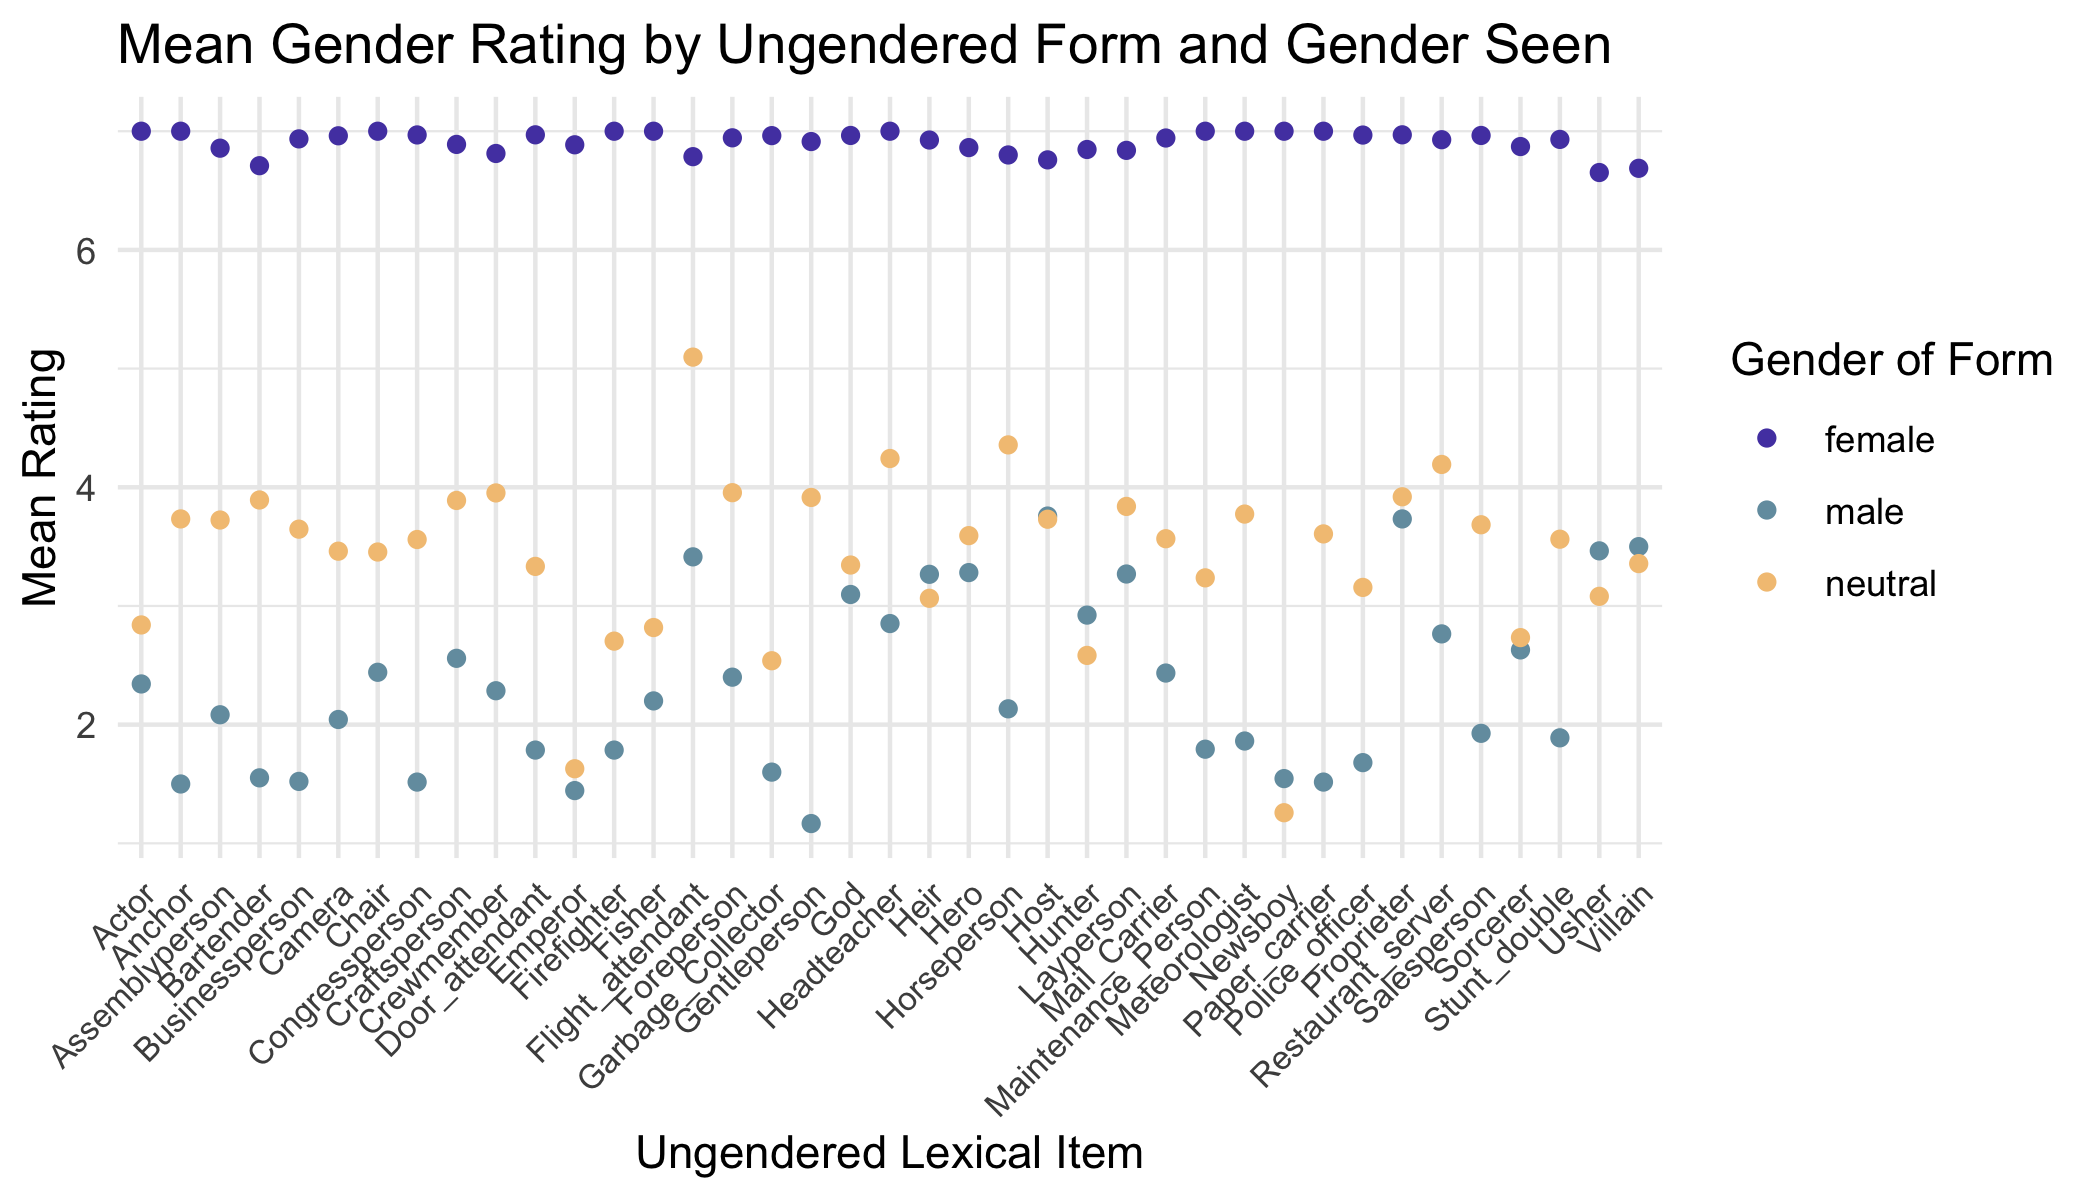
\includegraphics[scale=0.2]{norming_values.png}
		\caption{Mean gender ratings for the ~80 items in the norming study}
	\end{figure}
	
	\begin{figure}[h!]
		\centering
		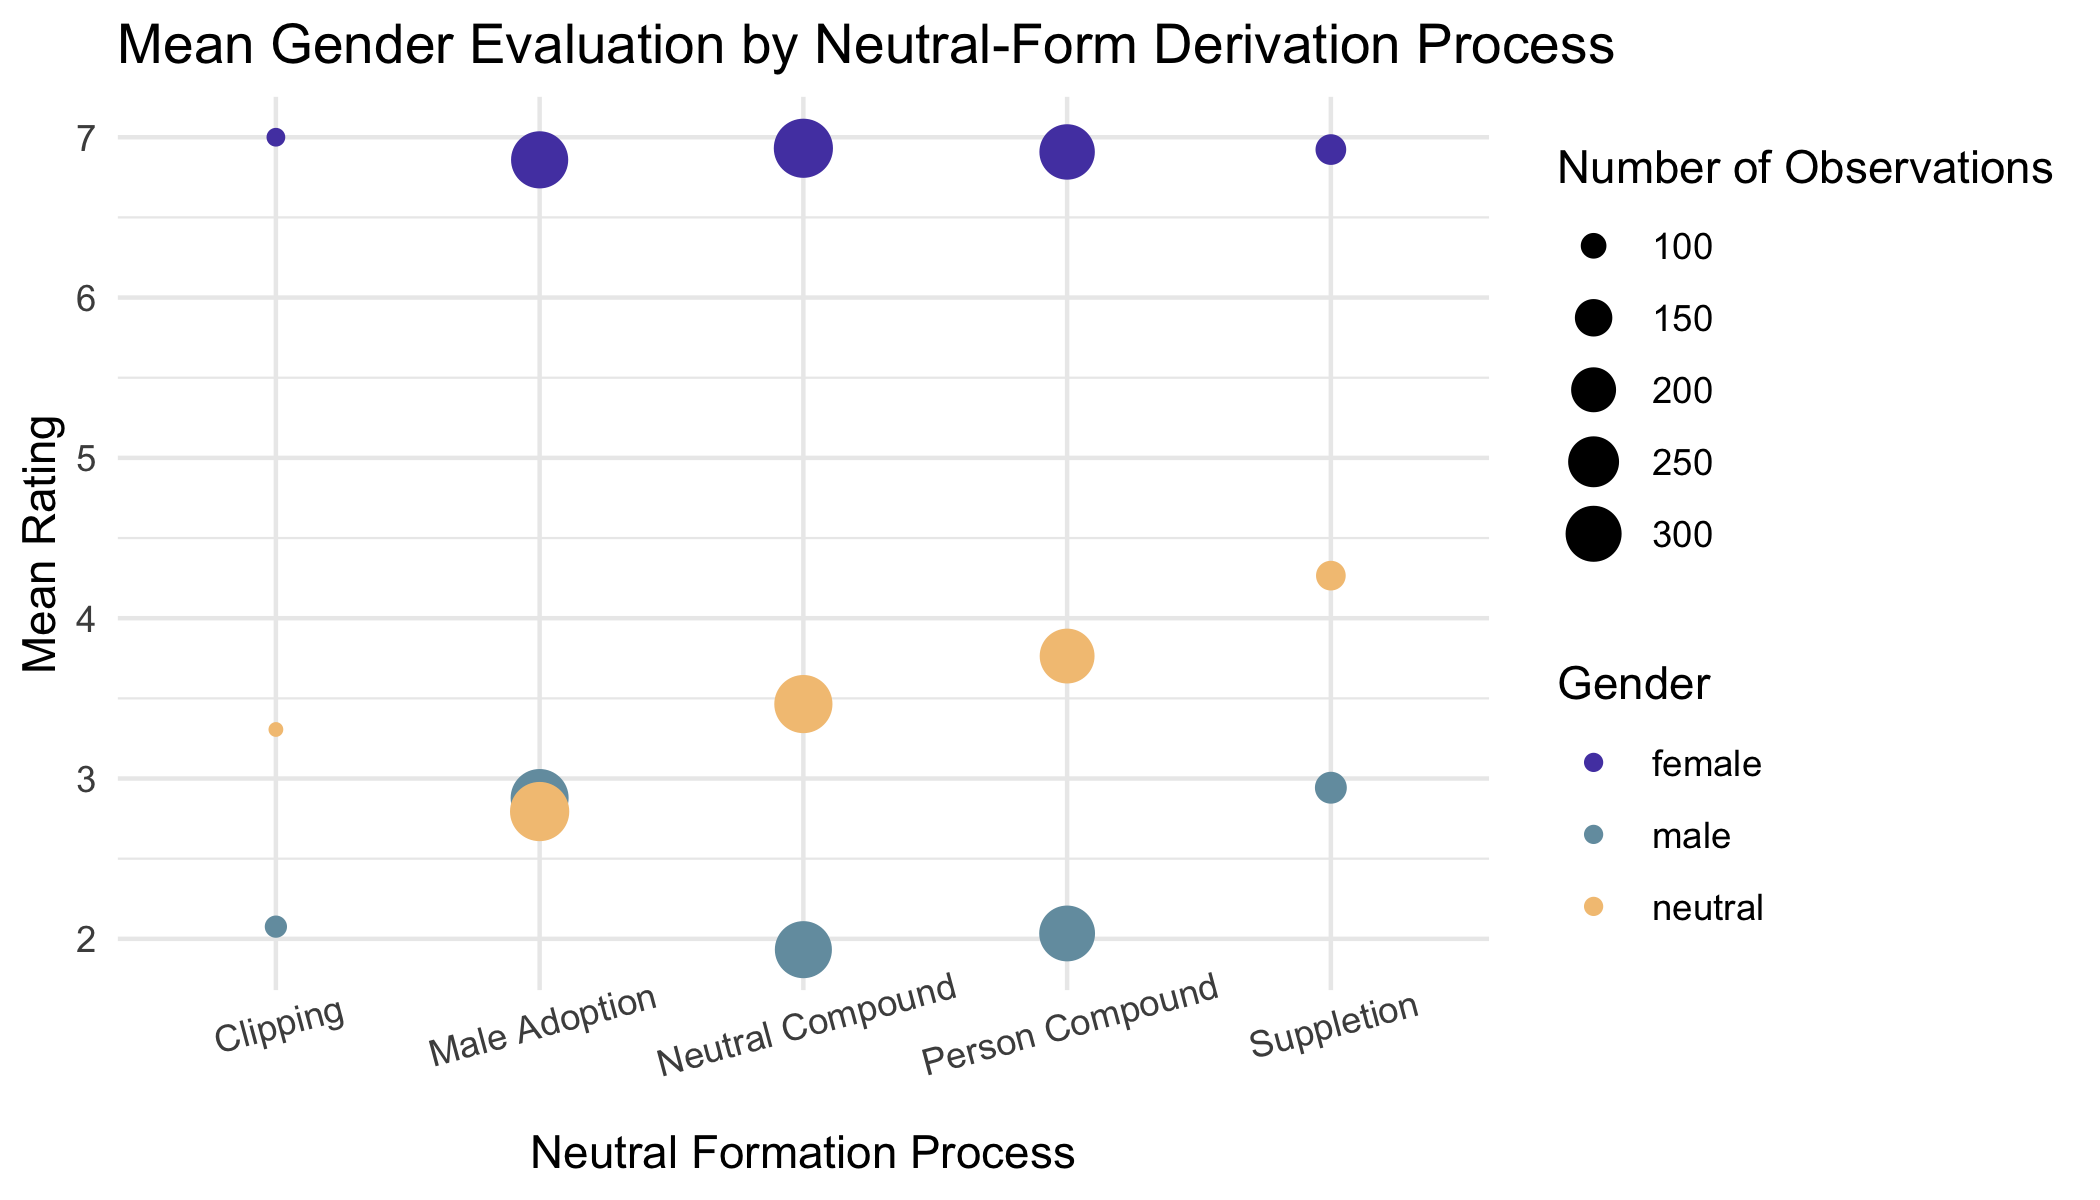
\includegraphics[scale=0.2]{norming_deriv.png}
		\caption{Mean gender ratings by morphological process of gender-neutral formation}
	\end{figure}
	
	\newpage
	\section{Experiment 1: Production}
	
	\subsection{Methods}
	
	\subsubsection{Participants}
	
	\subsubsection{Materials}
	
	\subsubsection{Procedure}
	
	\subsection{Results}
	
	\begin{figure}[h!]
		\centering
		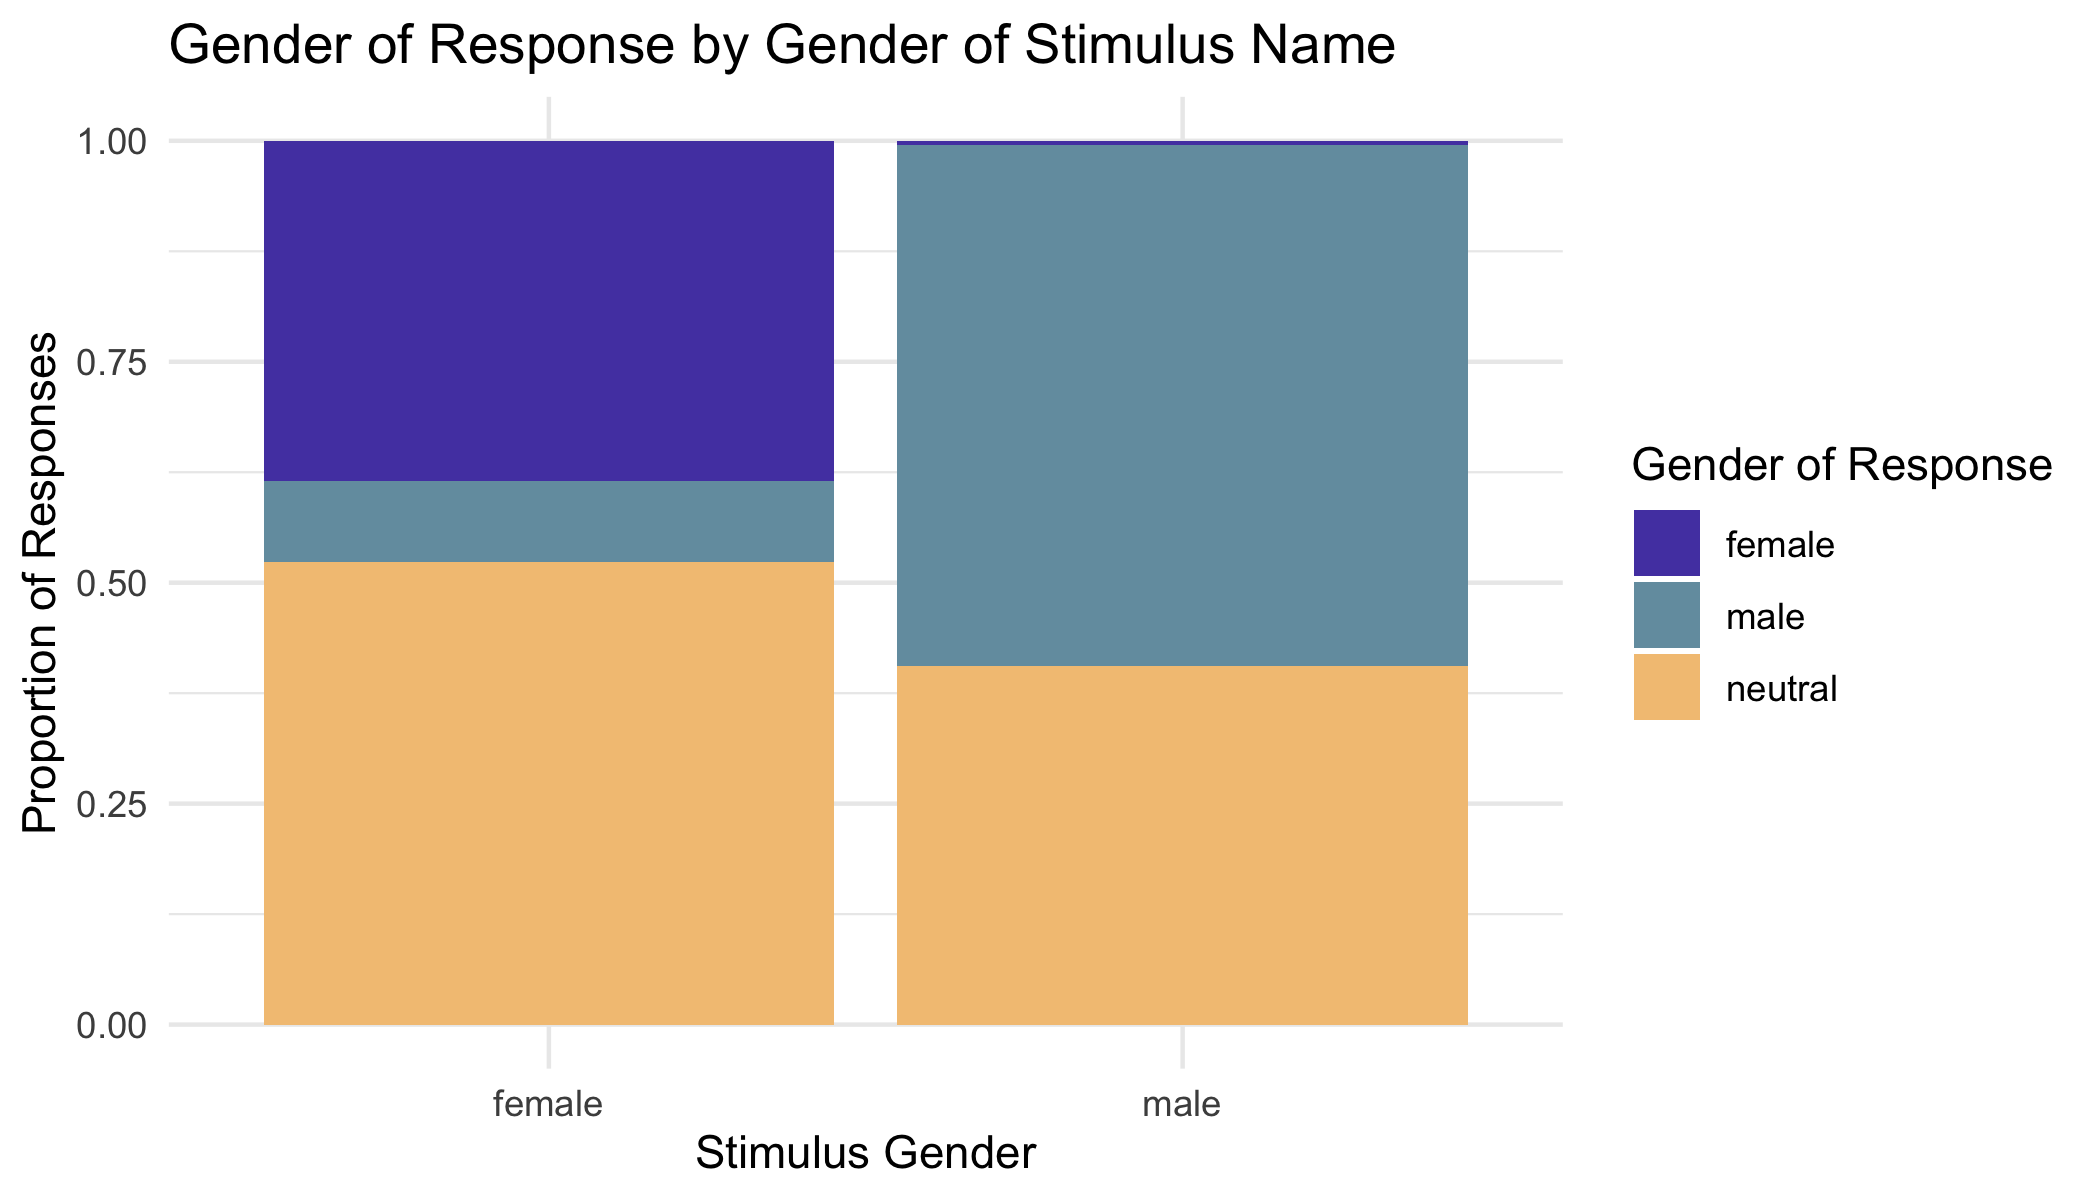
\includegraphics[scale=0.2]{prod_results_cumulative.png}
		\caption{Proportions of genders among produced responses in compound critical items}
	\end{figure}

	\begin{figure}[h!]
	\centering
	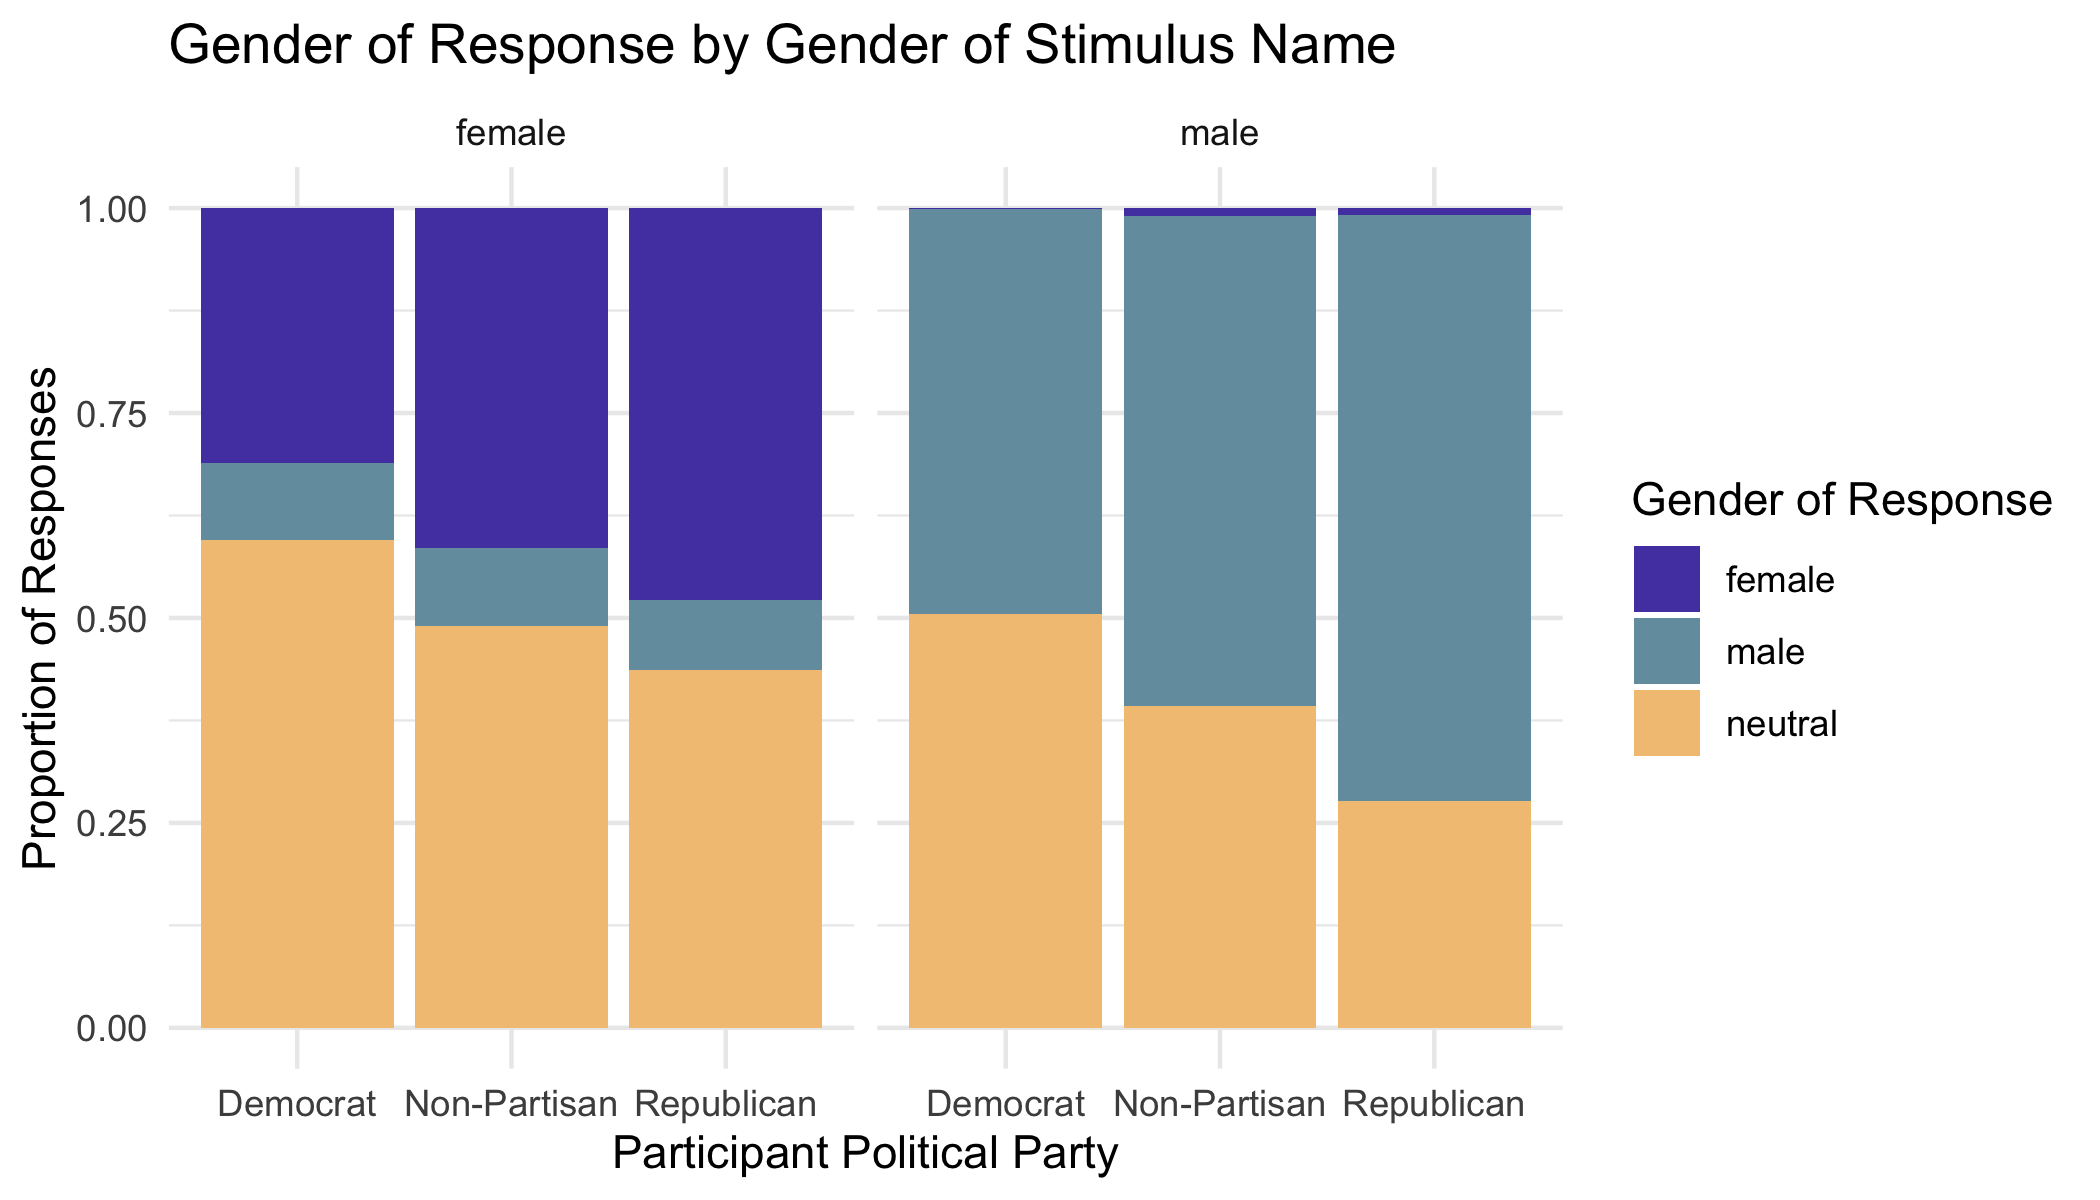
\includegraphics[scale=0.2]{prod_comp_party.png}
	\caption{Proportions of genders among produced responses in compound critical items}
	\end{figure}

	\begin{figure}[h!]
	\centering
	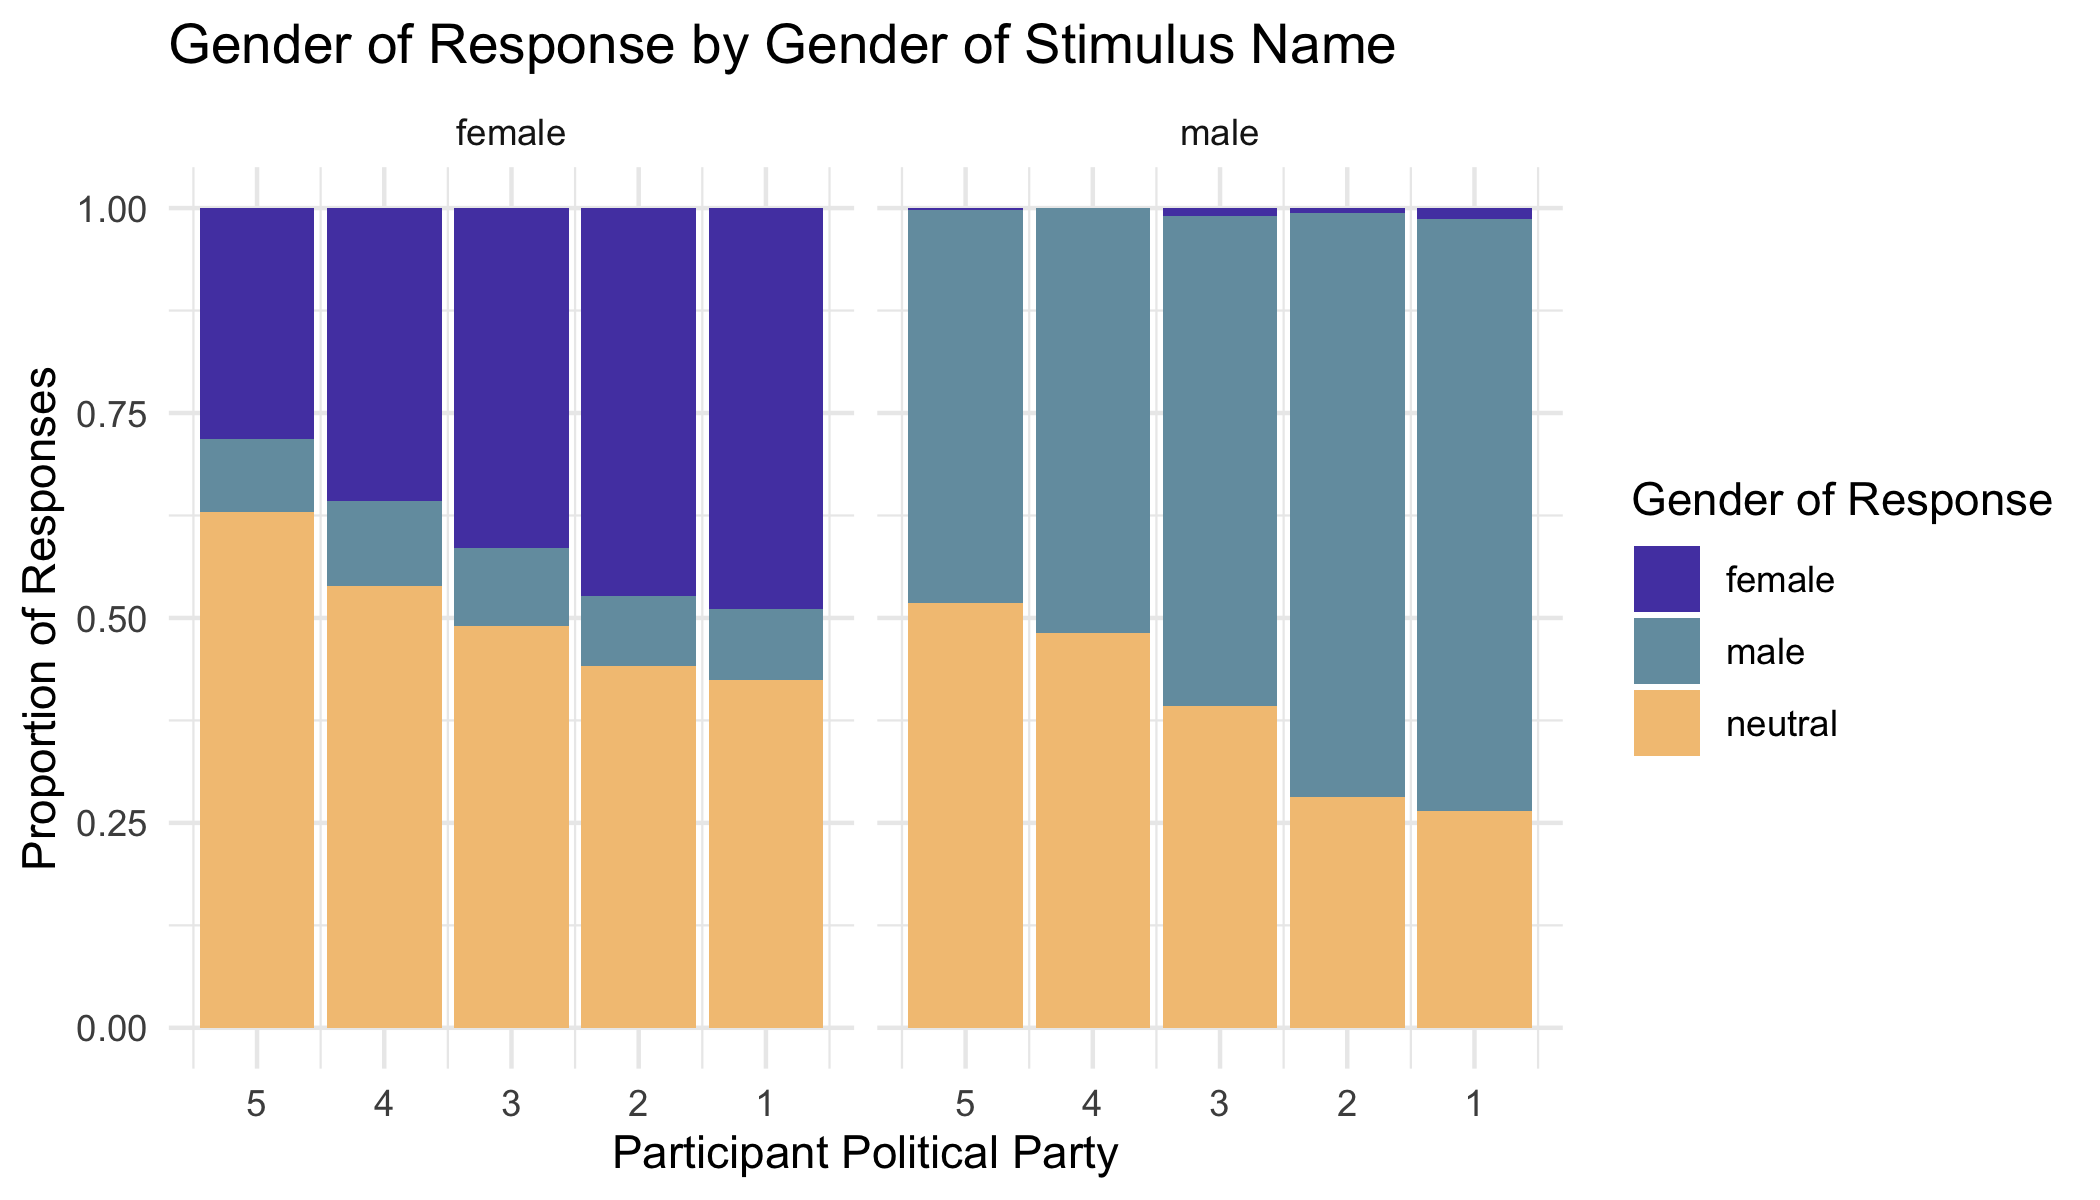
\includegraphics[scale=0.2]{prod_comp_ideo.png}
	\caption{Proportions of genders among produced responses in compound critical items}
	\end{figure}
	
	\newpage
	\section{Experiment 2}
	
	\subsection{Methods}
	
	\subsubsection{Participants}
	
	\subsubsection{Materials}
	
	\begin{table}[h!]
		\centering
		\begin{tabular}{l|l}
			\textbf{Condition} & \textbf{Example Stimulus}\\
			\hline
			Male-Congruent & \textit{David is a congressman from Virginia. He likes cycling.} \\
			Male-Neutral & \textit{David is a congressperson from Virginia. He likes cycling.} \\
			Female-Congruent & \textit{Sally is a congresswoman from Virginia. She likes cycling.}\\
			Female-Neutral & \textit{Sally is a congressperson from Virginia. She likes cycling.}
		\end{tabular}
		\caption{Example stimuli from experiment}
		\label{Table1}
	\end{table}
	
	\subsubsection{Procedure}
	
	\subsection{Results}
	
	\newpage
	\section{Experiment 2.5}
	
	\subsection{Methods}
	
	\subsubsection{Participants}
	
	\subsubsection{Materials}
	
	\subsubsection{Procedure}
	
	\subsection{Results}
	
	\newpage
	\section{Experiment 3}
	
	\subsection{Methods}
	
	\subsubsection{Participants}
	
	\subsubsection{Materials}
	
	\subsubsection{Procedure}
	
	\subsection{Results}
	
	\newpage
	\section{Analysis}
	
	\newpage
	\section{Discussion}
	
	\subsection{Limitations}
	
	\subsubsection{Demographic Limitations}
	\textbf{Political Skew} \\
	\linebreak
	\textbf{Gender Skew (TikTok)}
	
	\subsubsection{Stimuli Limitations}
	\textbf{Semantic Inconsistencies} \\
	\linebreak
	\textbf{Ordering of Experiment Parts}\\
	\linebreak
	\textbf{Low-Frequency Items}\\
	\linebreak
	\textbf{White Names}
	
	\subsubsection{Analysis Limitations}
	\textbf{Age-Ideology Confound}
	
	\subsection{Future Directions}
	
	\begin{itemize}
		\item Crossing raced names with gendered name
	\end{itemize}
	
	\newpage
	\section{Conclusion}
	
	\newpage
	
	\printbibliography
	
\end{document}